\section{Learning to describe new objects from corpora}
\label{sec:learning}

In the previous section we presented an algorithm that assumes that each relation R 
used in a referring expressions has a known probability of use R.\puse. In this section, 
we describe how to calculate these probabilities from corpora.  
The general set up is the following: we assume available a corpus of REs associated 
to different scenes that are prototypical of the domain in which the GRE algorithm will have to operate.   
We show first how to calculate R.\puse\ values for those scenes for which a corpus of REs is available.  
We then show how to generalize these values to 
other scenes in the domain, using a machine learning algorithm. We will exemplify the methodology using 
the TUNA-corpus that will be introduce in the Section~\ref{sec:tuna}.

\subsection{The TUNA-corpus: A corpus of referring expressions}
\label{sec:tuna}
%\usepackage{wrapfig}
%\begin{wrapfigure}{r}{40mm}
The ASGRE Challenge used the TUNA Corpus (Gatt
et al., 2007), a set of human-produced referring expressions (REs) for entities in visual domains of
pictures of furniture or people. The corpus was
collected during an online elicitation experiment in
which subjects typed descriptions of a target referent
in a domain in which there were also 6 other entities distractors.
This corpus contains plural and singular parts. In this paper we will use the singular part like used for the ASGRE Challenge. Each scene contains the target and distractors with theirs properties, the RE given for a human, and a manual annotation of this.   
For the challenge 780 singular descriptions in the corpus were used, and divided
into 60\% training data, 20\% development data and
20\% test data. Participants were given both input and output parts in the
training and development data, but just inputs in the
test data.

\begin{figure}[ht]
\begin{minipage}{0.50\linewidth}
\centering
%\hspace*{-.8cm}
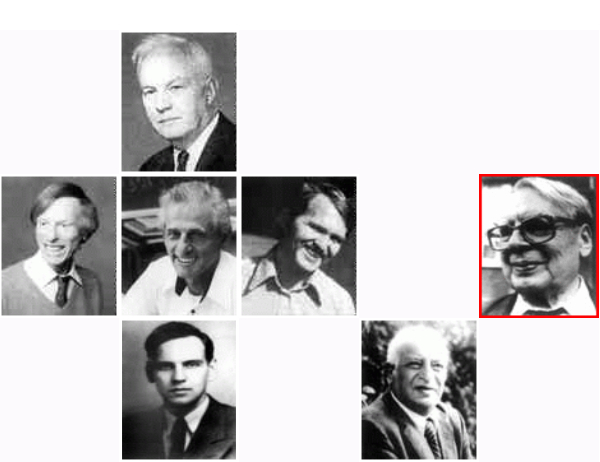
\includegraphics[width=\textwidth]{images/tuna-people.jpg}

%\vspace*{-.4cm}
\captionof{TUNA-corpus people scene}
\label{Tuna-people-scene}
\end{minipage}
%\hspace*{-0.21cm}
\begin{minipage}{0.5\linewidth}
\centering
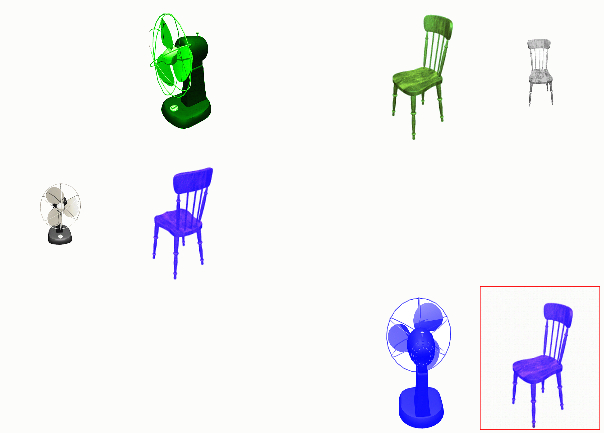
\includegraphics[width=\textwidth]{images/tuna.jpg}
%\vspace*{-.25cm}
%\vspace*{-.4cm}
\captionof{TUNA-corpus furniture scene}
%\captionof{figure}{Texto del pie de figura},
\label{Tuna-furniture-scene}
\end{minipage}
%\end{figure}
\end{figure}
%\end{wrapfigure}
\subsection{Calculating \puse\ when a corpus for the scene is available}

Suppose we want to automatically generate REs for target $t$ in a given scene, and that we do have available a corpus $C$ for scenes similar    
of REs for $t$ in that scene (this is exactly the kind of information we find in the TUNA-corpus).  
We use the models provided by TUNA as input of our algorithm.  
Then we estimate the value of \puse\ for each of the relations in the model as the percentage of REs 
in which the relation appears. I.e., 
\begin{equation}\label{eq1}
R.\puse = \frac{\# \mbox{ of REs in $C$ in which R appears}}{\# \mbox{ of REs in $C$}}.
\end{equation}

\noindent
This estimation is overly simplified and, for example, it does not differentiate between the properties of a target and the 
properties of a landmark object used in a relational RE to complete the description of the target, but in this case people don't use too much descriptions of lansmarks. It is extremely easy 
to compute, and we will see in Section~\ref{sec:evaluation} that it already produces natural REs that match those found in the corpus. 

To clarify the computation of R.\puse\ and the model $\gM$ associated to each scene we list the required steps in detail, 
and discuss how we carried them out in the TUNA corpus:

ESTAS COSAS... YO LAS SACARIA...

\vspace*{-.4cm}
\begin{enumerate}
\item Tokenize the referring expressions and call the set of tokens $T$. In particular, multi-word expressions like ``on top of'' 
should be matched to a single token like \emph{ontop}.\\[-1.9em]

\item Remove hyperonyms from $T$. E.g., if both \emph{cube} and \emph{thing} appear in $T$, delete \emph{thing}.\\[-2em]

\item If the set of tokens obtained in the previous steps contains synonyms normalize them to a representative in the synonym class, 
and call the resulting set $\REL$; it will be the signature of the model $\gM$ used by the algorithm. E.g., the tokens \emph{little} 
and \emph{small} are both represented by the token \emph{small}.\\[-1.9em]

\item For each scene, define $\gM$ such that the interpretation $\interp{\cdot}$ ensures that all the REs in the corpus are REs in the model.
 E.g., the $\el$ formulas corresponding to the REs in Table~\ref{corpus-distribution} should all denote the target in the model $\gM$ 
depicted in 
Figure~\ref{Tuna-scene}.\\[-1.9em]

\item For each R $\in \REL$ compute R.\puse\ using~(\ref{eq1}).\\[-1.9em]

\end{enumerate}

Steps 1-5 above are easy to carry out (actually, the tokenization and normalization steps were already done in the TUNA corpus). 
Starting from the scene in Figure~\ref{Tuna-scene} and the corresponding corpus (PROBLEMA: TENEMOS UN SOLA RE...) shown in Table~\ref{corpus-distribution}, 
the resulting signature and their associated \puse\ are listed in the first three columns of Table~\ref{probability-of-use}. 

Notice that the values R.\puse\ obtained in this way should be interpreted as the probability of using R to describe the target in model 
$\gM$, and we could argue that they are correlated to the \emph{saliency} of R in the model.  

For that reason, for example, the value of \emph{chair}.\puse\ is (AGREGAR ACA), while the value of \emph{fan}.\puse\ is (AGREGAR ACA)  
These probabilities will not be useful to describe different targets in different scenes. We will see how we can use them to obtain
 values for new targets and scenes using a machine learning approach in the next section. Not surprisingly, using these values for 
R.\puse\ the REs generated most often by the algorithm can be found in the corpus. More interestingly, as we discuss in 
Section~\ref{sec:evaluation} the algorithm generates REs with a distribution that matches the one found in the corpus and, 
as Table~\ref{results-algo-fig3} shows, even the generated REs not found in the corpus are natural.    


\subsection{Calculating \puse\ for scenes without corpora for the target} \label{subsec:learning}

If there is no corpora that describes the target we can estimate the \puse~from corpora on a different scenes in the same domain. 


The learning was done with the machine learning toolkit WEKA~\cite{Hall:WEK09}, training on all minus one (the one for that we are learning) for all the scenes of the TUNA-corpus. We use linear regression to learn the function of \puse\ for each word in the signature. 
For a given scene, we replace the variables of the obtained function by the values of the features in the scene that we want to describe. 
We use simple features to obtain the function, all the features can be extracted automatically from the relational model and are listed 
in Table~\ref{features}.  

\begin{small}
\begin{table}[h!]
\begin{center}
\begin{tabular}{|l|p{10cm}|}
\hline
target & whether the target element has the property \\
\#rel-prop & number of properties and relations that the target has\\
\#rel & number of the relations that the target has \\
landmark & whether a landmark of the target has the property, an object is a landmark if there is a direct relation in the model 
between them \\
discrimination & 1 over the number of objects in the model that have the property \\
\hline
\end{tabular}
\caption{Features used for learning the \puse for each token in the signature of the scenes of the TUNA-corpus} 
\label{features}
\end{center}
\end{table}
\end{small}
Our feature set is intentionally simplistic in order for it to be domain independent. As a result there are some complex relations 
between characteristics of the scenes that it is not able to capture. The most important characteristic of our domain is that we are not able 
to learn, and has an impact in our performance, we show that we couldn't learn the dependency of dimension-x and dimension-y, it mean, when a person adds dimension-x is highly probably that he includes dimension-y in his referring expression.
\begin{table}[h!]
\begin{center}
\begin{tabular}{|l|c|c|c|c|}
\hline
Token & Model Fig 3 \puse & Learned Fig 3\puse & Model Fig 13 \puse & Learned Fig 13 \puse \\
\hline
ball & 1.0 & 1.0 & 1.0 & 1.0 \\
cube & 1.0 & 1.0 & 1.0 & 1.0 \\
green & 0.978 & 0.993 & 1.0 & 0.9875 \\
small & 0.257 & 0.346 & 0.0428 & 0.1993 \\
on-top & 0.178 & 0.179 & 0 & 0\\ 
blue & 0.15 & 0.124 & 0.064 & 0.1353 \\
large & 0.107 & 0.03 & 0.307 & 0.7378 \\
left & 0.007 & 0.002 & 0 & 0.0024 \\
top & 0.007 & 0 & 0 & 0 \\
right & 0 & 0.001 & 0.064 & 0.0005 \\
left-of & 0 & 0 & 0 & 0 \\
right-of & 0 & 0 & 0.064 & 0.1023 \\
below-of & 0 & 0 & 0 & 0 \\
\hline
\end{tabular}
\caption{Probabilities of use of the tokens from the corpora in Table~\ref{Tuna-scene}} 
\label{probability-of-use}
\end{center}
\end{table}

\textit{Using} linear regression we are able to learn interesting characteristics of the domain. To start with, it learns known facts such that the 
saliency of a color depends strongly on whether the target object is of that color, and it does not depend on its discrimination power 
in the model. Moreover, (VER SI DEJAMOS ESTO) it learns that the on-top relation is used more frequently than the horizontal relations (left-of and right-of) 
which confirms a previous finding reported in~\cite{viet:gene11}. Finally, it learned a surprising fact of the TUNA corpus
 (not found by previous work), that is that size is used more frequently in an overspecified manner(VERIFICAR SI ESTO SE CUMPLE EN TUNA) when the target and landmark share the
 size. (REESCRIBIR ESTA PARTE, LA NOCION DE LANDMARK NO ES TAN USADA EN TUNA)Size was used in overspecified REs when in 49\% of the descriptions for scenes where target and landmark shared the size, and 25\% 
of the time when target and landmark did not share the size. This can be explained by the observation that if landmark and target share a
 property, this property is more salient. 

